\documentclass[11pt,a4paper]{article}

\usepackage[utf8]{inputenc}
\usepackage[T1]{fontenc}
\usepackage{lmodern}
\usepackage{amsmath,amssymb}
\usepackage{booktabs}
\usepackage{graphicx}
\usepackage{pgfplots}
\pgfplotsset{compat=1.18}
\usepackage{hyperref}
\usepackage{xcolor}
\usepackage{geometry}
\geometry{margin=2.5cm}

\hypersetup{colorlinks=true, linkcolor=blue!60!black, citecolor=blue!60!black, urlcolor=blue!60!black}

\title{3DFC: A Lossless Cold-Archive Container for Render Frame Sequences}
\author{}
\date{\today}

\begin{document}
\maketitle

\begin{abstract}
Render pipelines routinely produce tens of thousands of near-duplicate PNG
frames that must be retained long after a project wraps, yet no widely used
archival format is designed for this workload: still-image codecs ignore
temporal redundancy, video codecs rarely preserve alpha losslessly, and generic
archivers cannot exploit frame-to-frame similarity. This paper presents 3DFC, a
single-file container for PNG frame sequences that combines per-group adaptive
encoding (tile-sparse differencing with zstd, or lossless H.264 with a separate
alpha stream), byte-exact passthrough for incompressible content, per-frame
integrity hashes, random access by frame index, and resumable multi-step
encoding. On 2,000 real-world 640$\times$360 frames, 3DFC reduces 401.9\,MB to
185.7\,MB (53.8\% saved) while restoring every pixel, including transparency,
bit-identically. A parallel implementation on a 32-thread workstation encodes
2.8$\times$ faster than the sequential baseline with byte-identical output.
\end{abstract}

\section{Introduction}
\label{sec:intro}

A finished 3D shot typically leaves behind its rendered frames: thousands of
individually compressed PNG files that differ only slightly from their
neighbours. Artists keep them because a client may request a re-render, a
single replacement frame, or a new edit months later. The storage cost is
severe, and the available tooling is a poor fit:

\begin{itemize}
  \item Still-image formats (PNG~\cite{png}, JPEG~XL lossless~\cite{jxl}) compress each
  frame in isolation and ignore temporal redundancy entirely.
  \item Video codecs with true inter-frame prediction (H.264, HEVC~\cite{hevc}, AV1~\cite{av1})
  operate in YUV colour spaces; the RGB$\to$YUV$\to$RGB round trip is not
  bit-exact, and alpha support in lossless profiles is inconsistent.
  \item Generic archivers (zip, tar+zstd) treat frames as opaque blobs and miss
  pixel-level similarity.
\end{itemize}

3DFC is a container and toolchain built specifically for this cold-storage
workload: write once, verify, delete the originals, and restore all frames, one
frame, or an arbitrary inclusive range on demand. Its guarantees are narrow and
explicit: every restored \emph{pixel} (straight-alpha NRGBA, 8-bit/channel) is
identical to the source; 16-bit content is stored untouched. File-level
metadata outside the pixel buffer is not preserved.

The contributions of this paper are the container overview
(Section~\ref{sec:format}), the hybrid per-group encoding policy with a
never-worse guarantee (Section~\ref{sec:design}), the resumable and crash-safe
write path (Section~\ref{sec:resume}), and measured results on real footage
(Section~\ref{sec:eval}). The normative byte-level specification lives in the
companion \texttt{SPEC.md}.

\section{Related work}
\label{sec:related}

PNG~\cite{png} combines row filtering with DEFLATE~\cite{deflate}: excellent for single
images, blind to sequences. FFV1~\cite{ffv1} is a lossless intra-frame codec
supporting RGBA, but as an intra-only codec it captures no temporal redundancy.
Lossless H.264 (notably the RGB variant \texttt{x264rgb} at \texttt{qp~0})
preserves RGB values exactly and performs inter-frame prediction, but carries
no alpha channel, forcing a two-stream construction as adopted here. General
purpose compressors such as zstd~\cite{zstd} are used by 3DFC as the entropy
stage rather than as the whole solution. Content-defined archival with
deduplication and integrity hashing follows standard practice; 3DFC applies it
at frame and GOP granularity instead of byte-chunk granularity.

\section{Container format}
\label{sec:format}

A \texttt{.3dfc} file (format version~1) holds a fixed-size header, a sequence
of typed packets, the original filenames, a per-frame index giving $O(1)$
random access, and a trailing footer with the section offsets. Packets carry
keyframes, tile-sparse predicted frames, FFmpeg segments, or verbatim source
PNGs; every frame is covered by a truncated SHA-256 integrity hash. Frames are
numbered from~0 and restores reproduce the source naming. The complete
byte-level layout, flag definitions, hash rules, and compatibility requirements
are specified normatively in the companion \texttt{SPEC.md}; what follows
describes the design rationale rather than repeating it.

\section{Encoding design}
\label{sec:design}

\subsection{Segmentation}

The sequence is split into groups of pictures (GOPs, at most \texttt{gopMax}
frames, default~300). Tiles form a grid of $nx = \lceil W/T \rceil$ by
$ny = \lceil H/T \rceil$ cells for frame size $W \times H$ and tile edge $T$,
clipped at the frame borders. Let $\rho = C/(nx\cdot ny)$ be the fraction of
changed tiles between consecutive frames. A new group starts at a scene cut,
defined as $\rho > 0.85$ with a minimum group length of~8. Each group opens with a
keyframe, so groups are independent units for both parallel encoding and
parallel decoding. Filenames are ordered with natural (numeric-aware) sorting,
and numbering gaps or duplicates in a sequence are reported as warnings.

\subsection{Packet types}

\begin{description}
\item[GoI (0)] A keyframe: raw NRGBA bytes compressed with zstd at maximum
level.
\item[GoP (1)] A predicted frame: \texttt{count:u32le}, the changed tile
indices, then per-byte residuals
\begin{equation}
r_b = (c_b - p_b) \bmod 256,
\label{eq:residual}
\end{equation}
where $c_b$ and $p_b$ are corresponding bytes of the current and previous
frames, all zstd-compressed. Reconstruction applies
$c_b = (p_b + r_b) \bmod 256$. Unchanged tiles cost one bit in the change set.
\item[FF (2)] An FFmpeg segment for high-motion groups: \texttt{frames},
\texttt{rgbLen}, \texttt{alphaLen} (\texttt{u32le} each), followed by a
lossless \texttt{x264rgb} (\texttt{qp~0}) stream in a Matroska~\cite{matroska}
container and, when any frame carries
transparency, a lossless \texttt{x264} grayscale alpha stream. No YUV
conversion is used anywhere, preserving bit-exactness.
\item[Raw (3)] Source PNG bytes verbatim (16-bit content, or any group that
would otherwise grow).
\end{description}

\subsection{Hybrid policy and the never-worse guarantee}

Each GOP independently selects its engine: groups with mean tile-change ratio
below~0.45 use the Go path; above it, the FFmpeg path (when available).
Crucially, an encoded group is kept only if it is smaller than the source PNG
bytes plus packet overhead; otherwise the originals are stored verbatim.
The archive is therefore \emph{never larger than the sources plus a small
index}, regardless of content. Alpha is handled in straight (non-premultiplied)
form throughout, since premultiplied rounding is lossy for semi-transparent
pixels.

\subsection{Integrity}

Every frame carries a truncated SHA-256 hash~\cite{sha2} of its exact pixels (or source
bytes for passthrough frames). The \texttt{verify} operation re-decodes the
entire archive and compares hashes, and must succeed before source material is
deleted.

\section{Crash safety and resumability}
\label{sec:resume}

Archives are written to a temporary file and atomically renamed on success, so
an interrupted run never corrupts an existing archive, and existing outputs
are never overwritten without an explicit flag. Restored frames are likewise
written atomically, with pre-flight checks for name collisions and existing
files.

With resume enabled, each completed GOP commits three things: the packet data
(synced), an append-only journal of index records (synced), and a JSON
checkpoint recording the next segment, data offset, entry count, a fingerprint
of the source frames (SHA-256 over names and file hashes), and the encoding
configuration. A later run validates the fingerprint and configuration before
continuing from the last committed group; mismatches abort rather than produce
a corrupt archive, and checkpoint state is removed after a successful commit.
The sidecar file layout and validation rules are specified in
\texttt{SPEC.md}.

\section{Implementation}

The reference implementation is ~3{,}000 lines of dependency-light Go. The
scan pass decodes each PNG once (fast paths avoid generic colour conversion
for the common RGBA/NRGBA cases); independent GOPs are then encoded on a
worker pool capped to avoid zstd memory-bandwidth contention, with at most two
concurrent FFmpeg processes. Full restores and verifications decode GOPs in
parallel; single-frame and small-range operations stay sequential. All progress
callbacks are serialized and monotonic across the scan and encode phases.

\section{Evaluation}
\label{sec:eval}

\subsection{Method}

All figures below were produced by the tool itself (\texttt{archive},
\texttt{verify}, \texttt{benchmark}); every archive compared was verified and
restored pixel-identically. The footage set is the first 2{,}000 frames of a
640$\times$360 H.264 source (24\,fps), decoded once to PNG (401.9\,MB total).
For an original size $O$ and archive size $A$ we report space saved
$S = 1 - A/O$, compression ratio $R = O/A$, and for timings the speedup
$T_{\text{seq}}/T_{\text{par}}$ between the sequential baseline and the
parallel implementation on identical output bytes. Timings are representative
wall-clock figures on a 32-thread AMD Ryzen~9 7945HX with warm file cache,
on one footage set plus small synthetic sequences; they characterize this
workload, not a general benchmark suite.

\subsection{Compression}

\begin{table}[h]
\centering
\begin{tabular}{@{}lrrrr@{}}
\toprule
Content & Source & Archive & Saved & Mix \\
\midrule
Real footage, 2000 fr. & 401.9\,MB & 185.7\,MB & 53.8\% & Go~481 / FF~1478 / raw~41 \\
Static synthetic, 30 fr. & 65\,KB & 7\,KB & 89.7\% & Go only \\
Noisy footage, 100 fr. & 1.36\,MB & 1.4\,MB & passthrough & raw (never worse) \\
Mixed + alpha, 12 fr. & 5\,KB & 6\,KB & $-11$\% & metadata dominates at toy scale \\
\bottomrule
\end{tabular}
\caption{Measured compression. The 2000-frame run used default settings.}
\label{tab:compression}
\end{table}

Table~\ref{tab:compression} confirms the design intent: static content
collapses, mixed real footage roughly halves, and incompressible input falls
back to passthrough. A 12-frame cross-backend trial (Go, FFmpeg, auto) produced
byte-identical archives across equivalent configurations with all verifications
passing.

\begin{figure}[h]
\centering
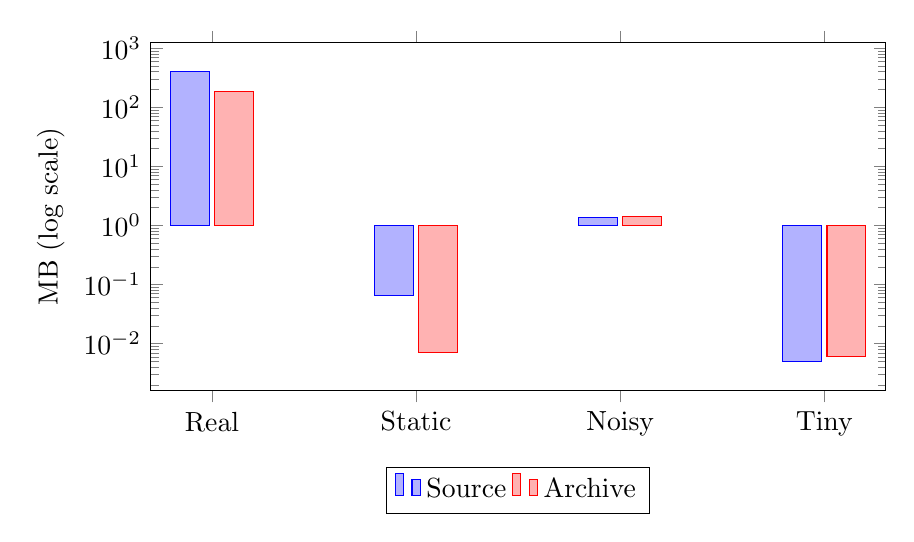
\begin{tikzpicture}
\begin{axis}[
  ybar, bar width=14pt,
  symbolic x coords={Real,Static,Noisy,Tiny},
  xtick=data,
  ylabel={MB (log scale)},
  ymode=log, log basis y=10,
  legend style={at={(0.5,-0.22)}, anchor=north, legend columns=-1},
  width=0.9\linewidth, height=6cm,
]
\addplot coordinates {(Real,401.9) (Static,0.065) (Noisy,1.36) (Tiny,0.005)};
\addplot coordinates {(Real,185.7) (Static,0.007) (Noisy,1.4) (Tiny,0.006)};
\legend{Source, Archive}
\end{axis}
\end{tikzpicture}
\caption{Source vs archive size per dataset on a logarithmic scale
(Table~\ref{tab:compression}).}
\label{fig:compression}
\end{figure}

\subsection{Speed}

On a 32-thread AMD Ryzen~9 7945HX, 300 real 640$\times$360 frames, Go backend:

\begin{table}[h]
\centering
\begin{tabular}{@{}lrrr@{}}
\toprule
Operation & Sequential & Parallel & Speedup \\
\midrule
Archive, fast preset & 4.41\,s & 1.56\,s & 2.8$\times$ \\
Archive, max preset & 6.90\,s & 2.83\,s & 2.4$\times$ \\
Extract all & 1.89\,s & 0.95\,s & 2.0$\times$ \\
Verify & 0.39\,s & 0.25\,s & 1.6$\times$ \\
\bottomrule
\end{tabular}
\caption{Parallel vs sequential on identical output bytes.}
\label{tab:speed}
\end{table}

Profiling showed PNG colour conversion and per-byte buffer growth as the
dominant CPU costs (addressed with direct blits and preallocated delta
buffers), file-creation syscalls as the dominant system cost (addressed by
in-RAM GOP hand-off and packet staging), and zstd memory-bandwidth contention
beyond eight concurrent max-level encoders (addressed with a worker cap, so
encode workers are capped at eight with no measured gain beyond that point on
this machine).
The FFmpeg path is unchanged by parallelism, as x264~\cite{x264} already saturates cores.

\begin{figure}[h]
\centering
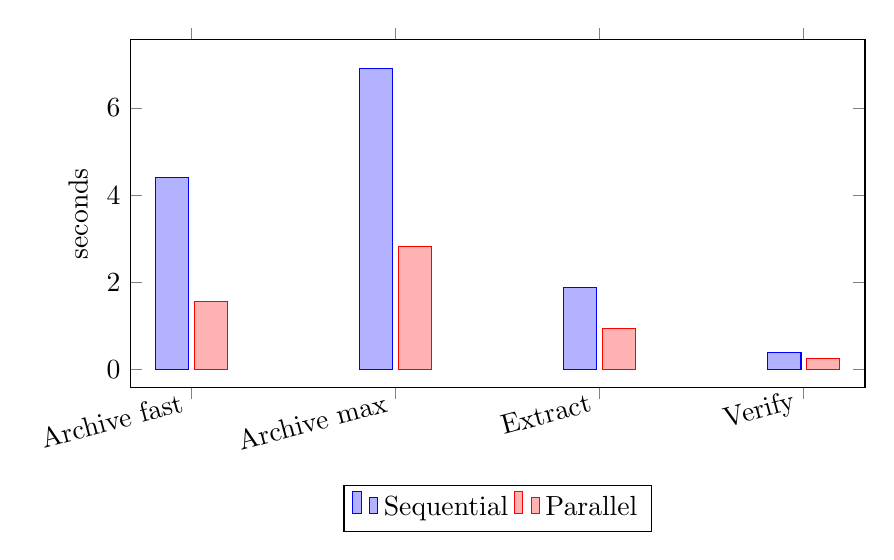
\begin{tikzpicture}
\begin{axis}[
  ybar, bar width=12pt,
  symbolic x coords={Archive fast,Archive max,Extract,Verify},
  xtick=data,
  xticklabel style={rotate=15, anchor=east},
  ylabel={seconds},
  legend style={at={(0.5,-0.28)}, anchor=north, legend columns=-1},
  width=0.9\linewidth, height=6cm,
]
\addplot coordinates {(Archive fast,4.41) (Archive max,6.90) (Extract,1.89) (Verify,0.39)};
\addplot coordinates {(Archive fast,1.56) (Archive max,2.83) (Extract,0.95) (Verify,0.25)};
\legend{Sequential, Parallel}
\end{axis}
\end{tikzpicture}
\caption{Sequential vs parallel wall-clock time per operation
(Table~\ref{tab:speed}).}
\label{fig:speed}
\end{figure}

\section{Limitations}

3DFC guarantees pixel identity, not file identity: restored PNGs are
re-encoded and PNG metadata (ICC profiles, gamma, text chunks) is not
preserved. Workflows depending on such metadata should test round-trips first.
Hashes are truncated to 64~bits (collision risk negligible for integrity
checking, unsuitable as content identifiers). Resume requires unchanged
sources and options by design.

\section{Conclusion}

3DFC demonstrates that a narrow, workload-specific container, combining
adaptive per-group lossless encoding, a strict never-worse fallback,
content fingerprinting, and crash-safe resumable writes, can halve real
render-footage archives with bit-exact pixels and practical restore
performance. Future work includes byte-exact PNG preservation modes and
optional near-lossless tiers for preview proxies.

\begin{thebibliography}{99}
\bibitem{png} ISO/IEC 15948:2004, \textit{Portable Network Graphics (PNG):
Functional specification}.
\bibitem{deflate} P.~Deutsch, \textit{DEFLATE Compressed Data Format
Specification version 1.3}, RFC~1951, 1996.
\bibitem{jxl} ISO/IEC 18181-1:2022, \textit{JPEG XL image coding system,
Part 1: Core coding system}.
\bibitem{hevc} G.~J.~Sullivan, J.-R.~Ohm, W.-J.~Han, and T.~Wiegand,
\textit{Overview of the High Efficiency Video Coding (HEVC) Standard},
IEEE Trans.\ Circuits Syst.\ Video Technol., vol.~22, no.~12, 2012.
\bibitem{av1} Alliance for Open Media, \textit{AV1 Bitstream \& Decoding
Process Specification}, 2018.
\bibitem{matroska} S.~Lhomme, M.~Bunkus, and D.~Rice, \textit{Matroska Media
Container Format Specifications}, RFC~9559, 2024.
\bibitem{zstd} Y.~Collet and M.~Turner, \textit{Zstandard Compression and the
\texttt{application/zstd} Media Type}, RFC~8878, 2021.
\bibitem{ffv1} M.~Niedermayer et al., \textit{FFV1 Video Coding Format},
IETF draft (versions 0--4).
\bibitem{sha2} NIST, \textit{Secure Hash Standard (SHS)}, FIPS PUB 180-4, 2015.
\bibitem{x264} VideoLAN, \textit{x264 H.264/AVC encoder},
\url{https://www.videolan.org/developers/x264.html}.
\end{thebibliography}

\end{document}
